% !TEX encoding = UTF-8 Unicode
% !TEX root = GANXXX.tex
% !TeX spellcheck = es_ES
%%=========================================	
\chapter{Estilo del texto}
En este capítulo se presenta el estilo general del texto que se desarrollará en formato de página A4. Se ha optado por un estilo Helvetica 11 pt (pudiendo optar por 12pt) a elección del alumno. Los márgenes recomendados son: superior 3 cm, inferior 1,5 cm, izquierdo 3 cm, derecho 1,75 cm. 

Esta plantilla de \LaTeX $ \ $ comienza cada capítulo en página impar y deja, si es necesario, la página anterior vacía.

Pueden desarrollarse los contenidos con distintos subapartados. Se trata en este documento de mostrar el formato elegido.
\section{El texto}
Se han de escribir las principales ideas, métodos, elementos de cálculo y de diseño utilizados. Recuerde que el número de páginas es limitado.
\subsection{Secciones y sub-secciones}	
No conviene expandir más del nivel de sub-sección la estructura del texto.

\section{Los elementos gráficos}
En este documento sólo se ofrece formato a las figuras y tablas.
\subsection{Figuras}
Las figuras se numeran automáticamente con el número de capítulo seguida del número de figura en orden creciente. Su título está centrado y debajo de la figura.


Se recomienda que las figuras vayan situadas adecuadamente en el texto. Recuerde que prioritariamente las figuras deben situarse en la parte alta de cada página. Sirva el siguiente ejemplo para ilustrar el formato de las figuras:
\begin{lstlisting}
\begin{figure}[H]
	\centering
	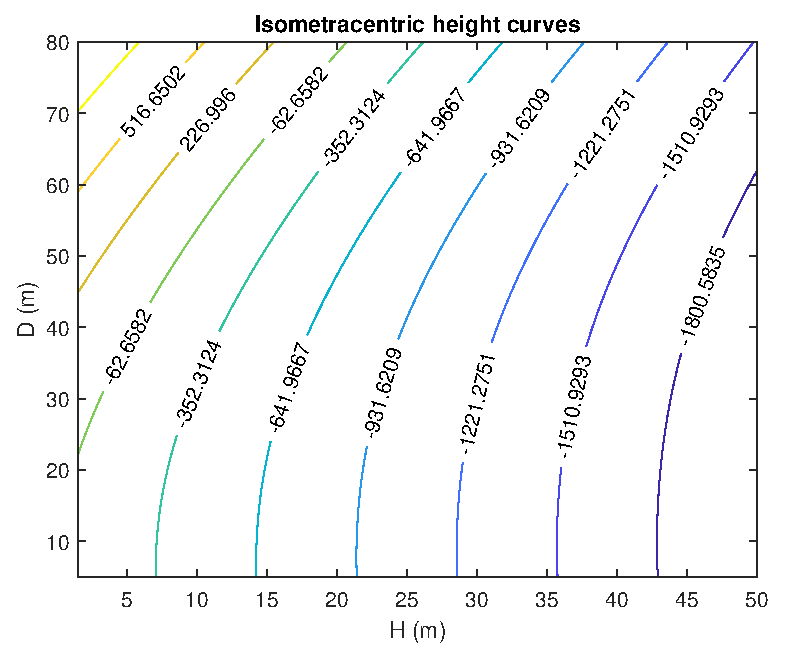
\includegraphics[width=0.8\textwidth]{images/figure_1.eps}
	\caption{La primera figura}
	\label{fig: isom}
\end{figure}
\end{lstlisting}
Generando el siguiente resultado:
\begin{figure}[H]
	\centering
	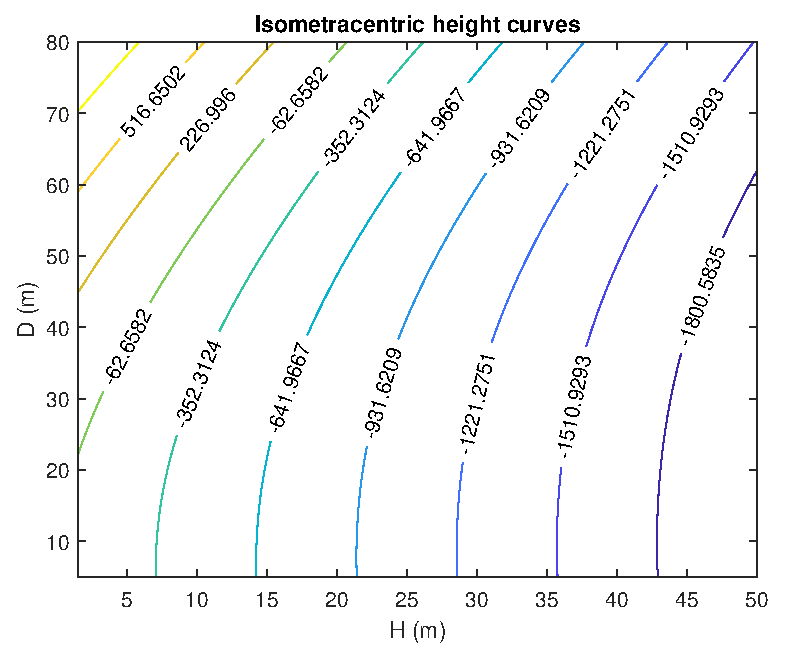
\includegraphics[width=0.8\textwidth]{images/figure_1.eps}
	\caption{La primera figura}
	\label{fig: isom}
\end{figure}

Recuerde insertar gráficas de alta calidad y a ser posible que se contraste bien lo que se quiere mostrar. No todos los documentos son impresos en color pese a las muy altas prestaciones gráficas de hoy en día.


Para colocar varias gráficas, se recurre al entorno \texttt{minipage}. 
\begin{lstlisting}
\begin{minipage}{0.5\textwidth}	
	\begin{figure}[H] 
		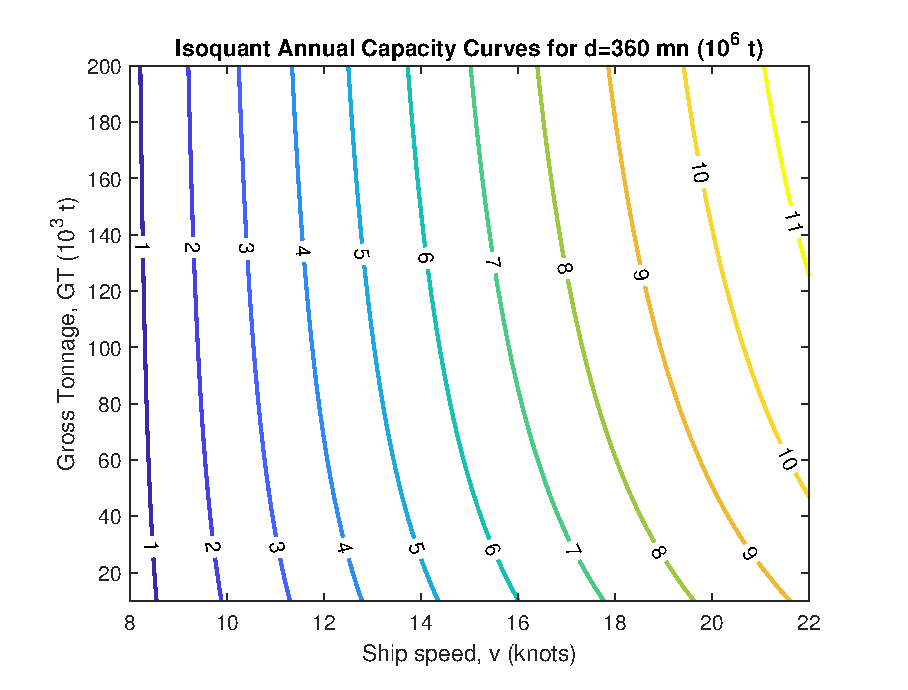
\includegraphics[width=1.00 \textwidth]{images/minipage1.eps}
		\caption{La segunda figura}
		\label{fig: minip}
	\end{figure}	
\end{minipage} \hfill \begin{minipage}{0.5\textwidth}	  
	\begin{figure}[H] 
		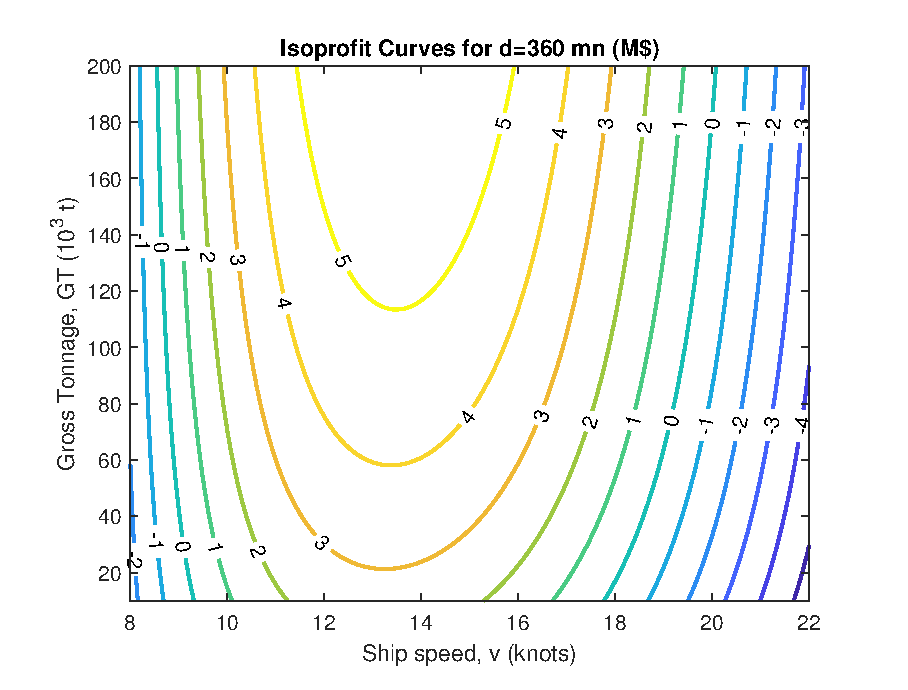
\includegraphics[width=1.00 \textwidth]{images/minipage2.eps}
		\caption{La tercera figura}
		\label{fig: minip2}
	\end{figure}
\end{minipage}
\end{lstlisting}

	\begin{minipage}{0.5\textwidth}	
		\begin{figure}[H] 
		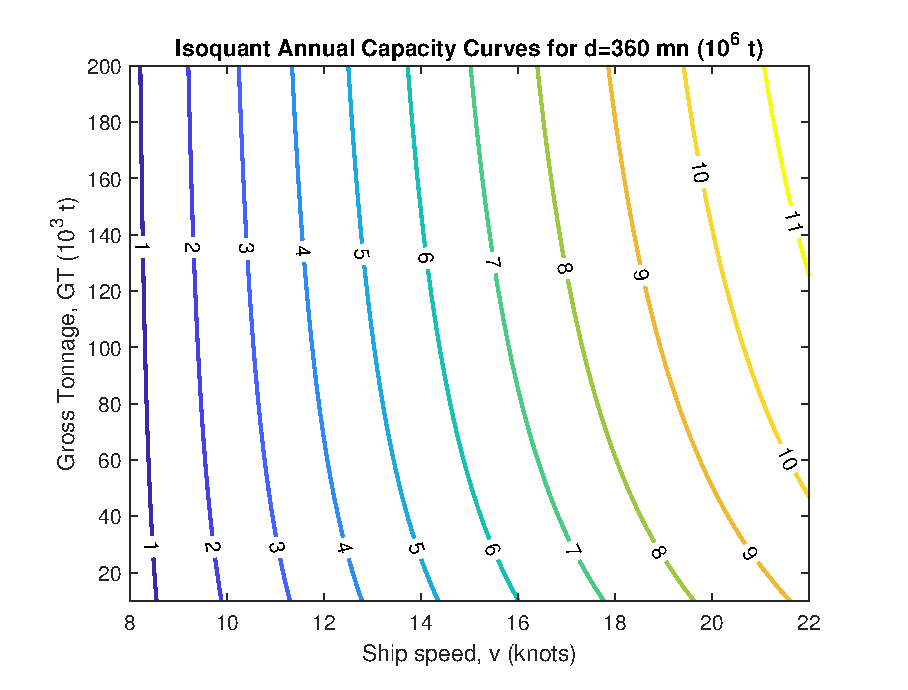
\includegraphics[width=1.00 \textwidth]{images/minipage1.eps}
		\caption{La segunda figura}
		\label{fig: minip}
		\end{figure}	
\end{minipage} \hfill \begin{minipage}{0.5\textwidth}	  
	\begin{figure}[H] 
		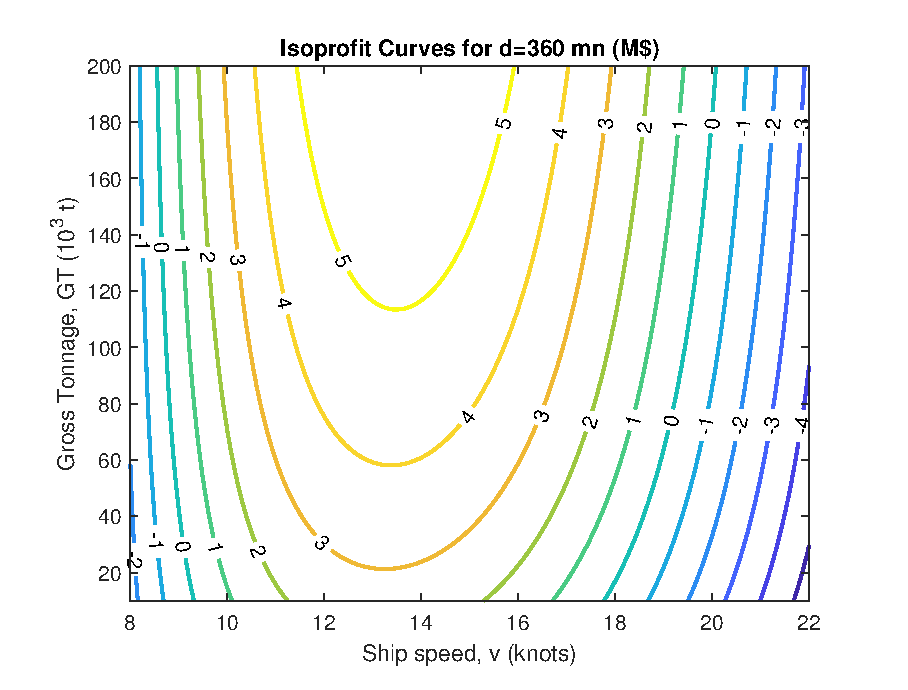
\includegraphics[width=1.00 \textwidth]{images/minipage2.eps}
		\caption{La tercera figura}
		\label{fig: minip2}
	\end{figure}
\end{minipage}


Se recuerda que ambas gráficas deben estar muy relacionadas para mostrarse juntas.
\subsection{Tablas}
Las tablas se numeran también con el número del capítulo seguido del número de tabla en orden creciente. El título está	 centrado y en la parte superior de la tabla. 


Se recomienda que las tablas tengan información concisa y bien estructurada. Sirva el siguiente ejemplo para ilustrar el formato de las figuras:
\begin{lstlisting}
% Table generated by Excel2LaTeX from sheet 'Hoja1'
\begin{table}[H]
\centering
\caption{Principales valores}
\begin{tabular}{lrr}
	\toprule
	Variable   & Valor &   Unidad \\ \midrule
	Potencia   &   1.2 &       MW \\
	Velocidad  &   2.3 &      m/s \\
	Impedancia &   0.3 & $\Omega$ \\ \bottomrule
\end{tabular}%
\label{tab: valores}%
\end{table}%
\end{lstlisting}
% Table generated by Excel2LaTeX from sheet 'Hoja1'
\begin{table}[H]
	\centering
	\caption{Principales valores}
	\begin{tabular}{lrr}
		\toprule
		Variable   & Valor &   Unidad \\ \midrule
		Potencia   &   1.2 &       MW \\
		Velocidad  &   2.3 &      m/s \\
		Impedancia &   0.3 & $\Omega$ \\ \bottomrule
	\end{tabular}%
	\label{tab: valores}%
\end{table}%
Una opción para realizar tablas es utilizar Excel y después generar el código mediante la macro \href{https://ctan.org/pkg/excel2latex?lang=en}{Excel2LaTeX}. Existen opciones similares para LibreOffice.
\subsection{Ecuaciones}
Para las ecuaciones, se pueden escribir en el modo ``en línea''  \lstinline!$c^2=b^2+a^2$!, produciendo el siguiente resultado $c^2=b^2+a^2$ o bien numerándose para luego ser referenciadas (ver Ecuación \ref{eq: ISE}), como se muestra a continuación.

\begin{lstlisting}
	\begin{equation}
	ISE=\int_{0}^{\infty} \left(\widetilde{f}(\tau)-f(\tau)\right) d\tau
	\label{eq: ISE}
	\end{equation}
\end{lstlisting}
\begin{equation}
	ISE=\int_{0}^{\infty} \left(\widetilde{f}(\tau)-f(\tau)\right) d\tau
	\label{eq: ISE}
\end{equation}
Existen numerosos recursos en línea para editar las ecuaciones fácilmente, se recomienda \href{http://www.hostmath.com/}{HostMath}.

\section{Algoritmos}
Para la exposición de un algoritmo u otro procedimiento que se requiera para la puesta en marcha, fabricación, proceso, etc. se puede recurrir al formato que se encuentra en el Anexo \ref{ch: A}. Nótese que no se recomienda incluir código de programación o similares en el cuerpo del documento.
\section{Otros elementos}
Se incluyen aquí otros elementos sujetos a formato como pueden ser los siguientes:


Listas enumeradas
\begin{enumerate}
	\item Primer elemento numerado.
	\item Segundo elemento numerado.
	\item ...
	\item hasta el último
\end{enumerate} 

Viñetas
\begin{itemize}
	\item Primer elemento numerado.
	\item Segundo elemento numerado.
	\item ...
	\item hasta el último
\end{itemize}